\chapter{A Chemical Data Assimilation Framework for Indoor Air Quality Assessment}

As described in the introduction, the COVID-19 pandemic has catalyzed global concern for indoor air quality. In order to provide actionable insights, a comprehensive analysis of the relevant chemistry is needed to establish how chemical constituents interact in indoor spaces. Much of outdoor air chemistry is driven by light; short wavelength photons can break bonds through photolysis and changing light conditions due to the rotation of the Earth introduce diurnal variations which drive relevant atmospheric reactions. Very little UV light makes it through building windows and into the indoor spaces. Additionally there is a large variability in indoor light sources including LED, fluorescent, incandescent and others which each have very different spectral properties. Therefore to establish a baseline for the relevant chemical processes indoors pertaining to air quality, we have developed an advanced sensing suite called the HEART chamber as described in chapter 2. By combining high quality measurements for a variety of source gases and aerosols together with detailed characterization of indoor photolysis we are able to produce rich data sets constraining the breadth of possible reactions in indoor spaces. Using this high quality data, we can then use techniques of data assimilation to constrain complicated chemical kinetics mechanism in order to infer the abundance of species that are too reactive to directly measure.

In this chapter we first introduce the relevant physics for reaction kinetics and photolysis which we will use in the construction and evaluation of our reaction mechanism models. Then we present preliminary results on a detailed evaluation of photolysis rates as well as initial measurements from our HEART chamber chemical kinetics evaluations using our data assimilation framework.

\section{Physics of Chemical Reactions: Chemical Reaction Kinetics}

\subsection{Overview}

Since the early successes of Newton's descriptions of mechanics by means of simple forces acting on masses, scientists have sought to understand the dynamics of chemical reactions in terms of the detailed microphysics of molecular collisions. As we shall see, this approach can be utilized productively to justify the complicated temperature and pressure dependence of the reaction rate coefficients of many elementary reaction. However, even when considering the asymmetric structure of many molecules, and therefore, the dependence on orientation at the collision site, kinetic theory alone is unable to model reaction rates in all relevant temperature and pressure regimes. To do this, one can utilize the modern treatment of \textit{Potential Energy Surface} (PES) theory together with the notion of short-lived, unstable intermediate reaction states to calculate reaction rate coefficient functions for specific reactants. \textit{Ab initio} solution of the Schrodinger equation for the relevant nuclear geometries ($3N$ reaction coordinates for $N$ atoms) together with scattering and spectroscopic methods as suggested by \cite{transition-state-spectroscopy-bimol} have led to significant improvements in our understanding of reaction dynamics.



\begin{figure}[h]
  \centering
  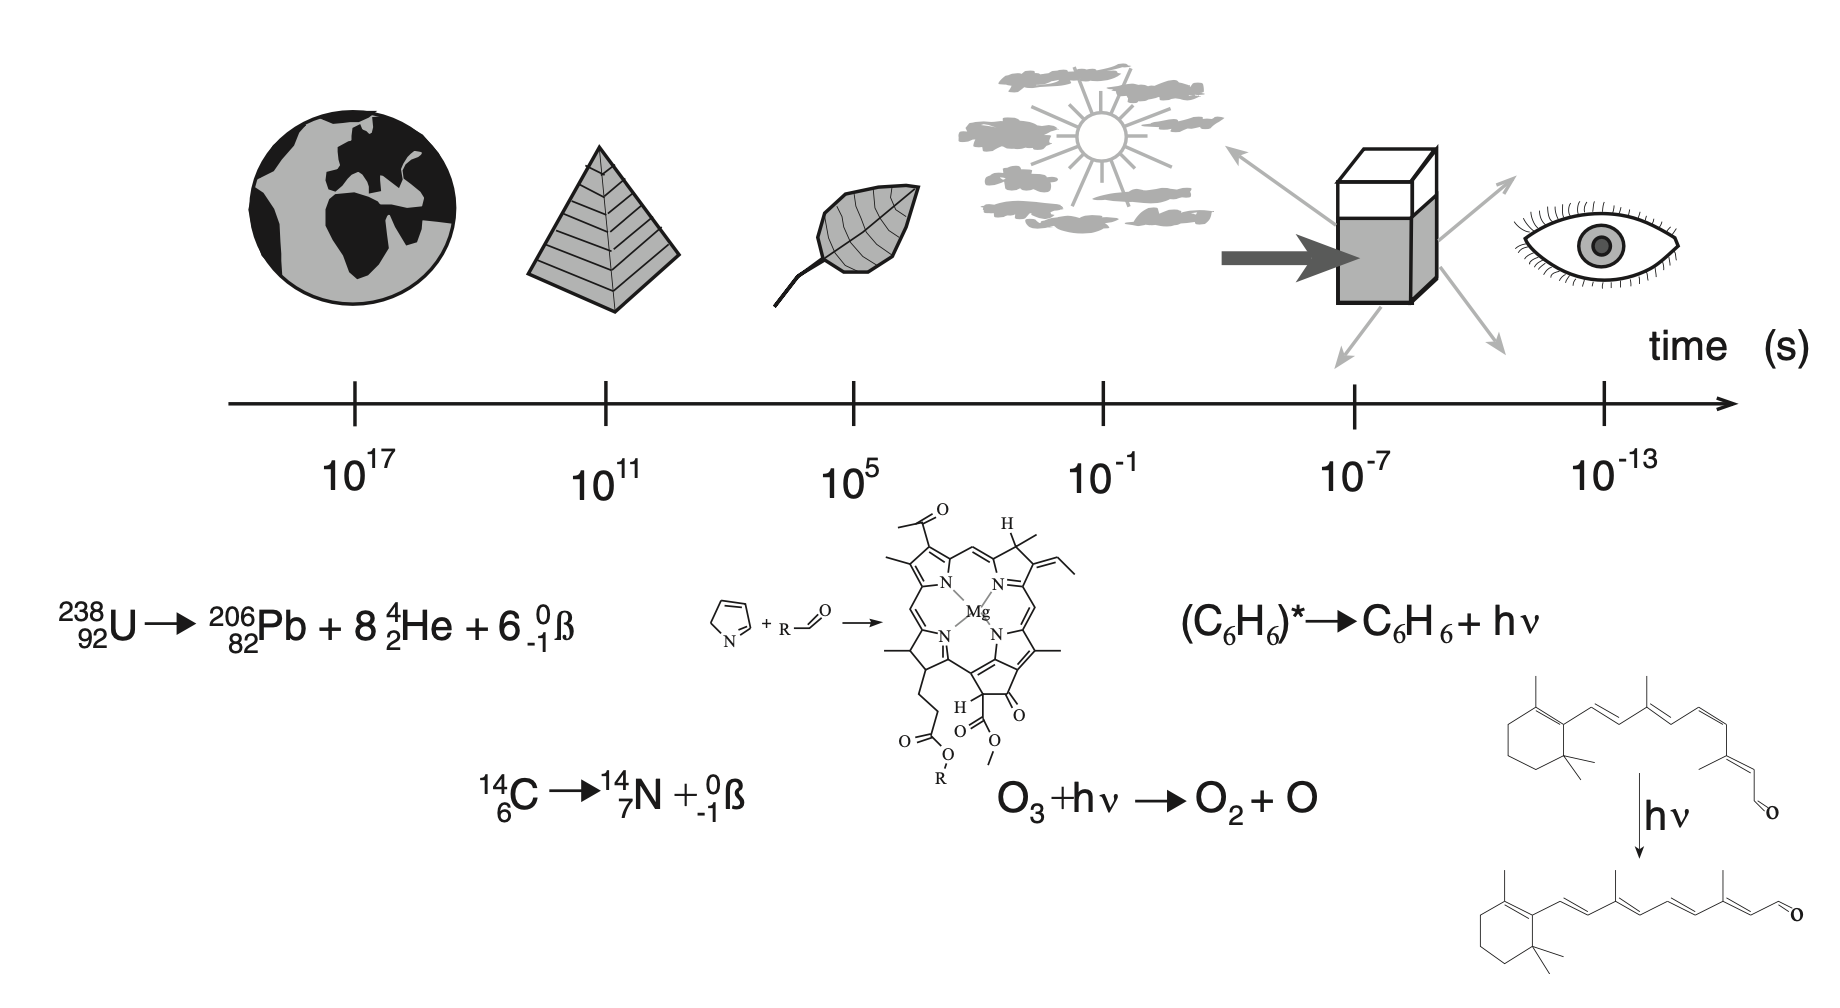
\includegraphics[width=0.85\textwidth]{introduction/reaction-timescales.png}
  \caption{An illustration of the broad range of reaction time scales from the long-lived nuclear decay to rapid degradation of molecules by photolysis. Figure taken from \cite{arnaut2006chemical}}
  \label{fig:reaction-timescales}
\end{figure}


However the computational complexity of this task makes it prohibitively expensive to perform at the scale required for our desired chemical mechanism which consists of many hundreds to thousands of reactants together with as many as 16,000 unique reactions. Therefore in the following discussion, we shall primarily utilize the kinetic theory to justify the functional form for \textit{most} rate coefficients with some reference to the extensions made by PES theory. We note that in practice, kinetic evaluations such as the periodic reports from the NASA Jet Propulsion Laboratory \cite{jpl-kinetic-evaluation-2020} utilize (justified) empirical fits to provide suggested functional forms for reaction rate coefficients.

\subsection{Chemical Equilibrium and the Law of Mass Action}

Before outlining the dynamics involved during complex chains of chemical reactions, it is worth spending some time to consider how we should treat chemical equilibrium. Usually in these scenarios we can not hold the internal energy fixed due to interactions with the environment, but rather, the temperature and pressure can often be treated as so. For example, we may be interested in gas-phase reactions occurring in ambient indoor air at or near standard temperature and pressure. In such scenarios, one finds the relevant potential energy to be the Gibbs, given by
\begin{equation}
  G = U - TS + PV,
\end{equation}
which is minimized in equilibrium under constant temperature and pressure.

This equation leads to the convenient thermodynamic identity
\begin{equation}
  dG = -SdT + VdP + \sum_i \mu_i dN_i
\end{equation}
from which we may identify the \textit{chemical potential} of the $i^{th}$ species as
\begin{equation}
  \mu_i  = \left(\frac{\partial G}{\partial N_i} \right)_{T,P,N_{j\neq i}}.
\end{equation}
The fact that each $\mu_i$ depends only on intensive state variables allows us to further simplify the relationship by considering what would happen were we to gradually increase the size of the system while maintaining the values of intensive parameters $T$, $P$, $\mu_i$. The result is G must increase in direct proportion to the increase in each $N_i$, that is:
\begin{equation}
  \label{eq:free-energy-definition}
  G = \sum_i \mu_i N_i.
\end{equation}
From equation \ref{eq:free-energy-definition} it is clear that the $\mu_i$ can be understood as molecular \textit{potentials} (i.e. chemical energy per molecule) in analogy to the notion of electric potential as a energy per unit charge.


For an ideal gas consisting of a single component we can combine equation \ref{eq:free-energy-definition} together with the identity
\begin{equation}
  V = \left(\frac{\partial G}{\partial P}\right)_{T,N}
\end{equation}
to obtain
\begin{equation}
  \left(\frac{\partial \mu}{\partial P}\right)_{T,N} = \left(\frac{\partial}{\partial P}\frac{G}{N}\right)_{T,N} = \frac{1}{N}\left(\frac{\partial G}{\partial P} \right)_{T,N} = \frac{V}{N} = \frac{kT}{P}
\end{equation}
so that by integration from a reference pressure, say $P_0= 1$ atm, we obtain the handy expression for the chemical potential
\begin{equation}
  \label{eq:mu-ideal}
  \mu(T,P) = \mu(T,P_0) + kT\ln(P/P_0)
\end{equation}
which we shall use again momentarily.

%% To understand what happens to $G$ at equilibrium where we know $dG=0$, let's now consider a homogeneous dilute mixture of a chemical species $B$ into species $A$. In the absence of $B$, we should have
%% \begin{equation}
%%   \label{eq:gibbs-A}
%%   G = N_{A}\mu_{0}(T,P)
%% \end{equation}
%% where $\mu_0$ denotes the chemical potential of the pure substance with just $A$. Adding a single particle of $N_{B}$ would then lead to an increase in free energy by some intrinsic amount $f(T,P)$ in addition to an increase from the added entropy due to the fact that we can place the particle (to a reasonable approximation) near anyone of the $N_{A}$ original particles. Therefore, we should expect an increase of
%% \begin{equation}
%%   dG = f(T,P) -T(k\ln(N_{A}))
%% \end{equation}

%% If we continue to add more particles until $N_{B}$, we will have added a total of $N_{B}$ contributions of $f(T,P)$ in addition to an entropy increase from an added multiplicity of states amounting to $N_{A}^{N_{B}}/N_{B}!$ or,
%% \begin{equation}
%%   \begin{aligned}
%%     dG &= N_{B}f(T,P) - N_{B}kT\ln(N_{A}) + kT\ln(N_{B}!) \\
%%     &\approx N_{B}f(T,P) - N_{B}kT\ln(N_{A}) + kTN_{B}(\ln(N_{B})-1) \qquad\text{(Stirling)}
%%     \end{aligned}
%% \end{equation}
%% putting this together with equation \ref{eq:gibbs-A}, we obtain
%% \begin{equation}
%%   G = N_{A}\mu_0(T,P) + N_{B}f(T,P) - N_{B}kT\ln(N_{A}) + N_{B}kT\ln(N_{B}) - N_{B}kT
%% \end{equation}

Returning now to the notion of chemical equilibrium, recall that we must have $dG=0$ so that $G$ is minimized. At constant temperature and pressure, this means
\begin{equation}
  0 = dG = -\cancel{SdT} + \cancel{VdP} + \sum_i \mu_i dN_i = \sum_i\mu_i dN_i
\end{equation}
and therefore, a generic reaction of the form
\begin{equation}
  \nu_1X_1 + \nu_2X_2 + \cdots \leftrightarrow \nu_3 X_3 + \nu_4 X_4 \cdots
\end{equation}
with chemical species $X_i$ and stoichiometric coefficients $\nu_i$ satisfies the condition that
\begin{equation}
  \nu_1\mu_1 + \nu_2\mu_2 + \cdots = \nu_3\mu_3 + \nu_4\mu_4 + \cdots.
\end{equation}

If we now make use of equation \ref{eq:mu-ideal} with the identification of $\mu^0 = \mu(T,P_0)$, then we obtain
\begin{equation}
  \sum_{i}^{\text{products}}\nu_i\mu_i^0 + \nu_i kT\ln(P_i/P_0) = \sum_{j}^{\text{reactants}} \nu_j\mu_j^0 + \nu_j kT\ln(P_j/P_0).
\end{equation}
collecting terms involving the $\mu^0_k$ to one side and multiplying through by Avogadro's constant, we obtain
\begin{equation}
  RT\ln\left(\frac{\prod\limits_j^{\text{reactants}}\left(\frac{P_i}{P_0}\right)^{\nu_i}}{\prod\limits_j^{\text{products}}\left(\frac{P_j}{P_0}\right)^{\nu_j}}\right) = R\left(\sum_j^{\text{reactants}}\nu_j\mu_j^0 -  \sum_i^{\text{products}} \nu_i\mu_i^0\right) = \Delta G^0
\end{equation}
so that by exponentiation, we arrive at the simple expression:
\begin{equation}
  \frac{\prod\limits_j^{\text{products}}\left(\frac{P_j}{P_0}\right)^{\nu_j}}{\prod\limits_i^{\text{reactants}}\left(\frac{P_i}{P_0}\right)^{\nu_i}} = \exp(-\Delta G^0/RT)
\end{equation}
which through further application of the ideal gas law yields
\begin{equation}
  \label{eq:law-of-mass-action}
  \boxed{\frac{\prod\limits_j^{\text{products}}\left(X_j\right)^{\nu_j}}{\prod\limits_i^{\text{reactants}}\left(X_i\right)^{\nu_i}} = K_{\text{eq}}}
\end{equation}
Here $K_{\text{eq}}$ is a temperature dependent constant called the \textit{equilibrium constant} for the reaction, and equation \ref{eq:law-of-mass-action} is called the \textit{law of mass action}. This expression indicates what we can expect to find if we allow our reactive system to proceed far enough to reach equilibrium. We shall later utilize this expression to perform a thermodynamic \textit{sanity check} as is described in \cite{boldi-thesis}. 


\subsection{Reaction Rate Laws}

Having established the expected behavior at equilibrium, our task now is to establish the correct dynamical laws describing the variety of reactions which take place. To begin, let us consider again a generic chemical reaction of the form
\begin{equation}
  \nu_{1}X_1 + \nu_{2}X_2 + \cdots \longrightarrow \nu_{3}X_3 + \nu_{4}X_4 + \cdots
\end{equation}

To describe the dynamical process of a reaction, we can introduce a parameter $\xi$ called the \textit{reaction extent} such that at any time we have
\begin{equation}
  \xi(t) = \frac{\lvert N_i(t) - N_i(0) \rvert}{ \nu_i}
\end{equation}
where $N_i(t)$ is the number  of the $i^{th}$ species and $\nu_i$ is the stoichiometric coefficient. The reaction rate is then easily understood as the rate of change of the reaction extent,
\begin{equation}
  r := \frac{d\xi}{dt} = \frac{1}{\nu_i}\left\lvert \frac{dN_i(t)} { dt} \right\rvert.
\end{equation}
Manipulating this expression to introduce the volume then leads us to
\begin{equation}
  r(t) = \frac{1}{\nu_i}\left\lvert\frac{dN_i}{dt}\frac{V}{V} \right\rvert = \frac{V}{\nu_i}\left\lvert \frac{d[X_i]}{dt} \right\rvert
\end{equation}
where $[X_i]$ denotes the concentration (number density) of the $i^{th}$ species participating in the reaction. All this is to say that upon rearranging the expression, we find
\begin{equation}
  \left\lvert \frac{d[X_i]}{dt} \right\rvert = \nu_i\frac{r(t)}{V} = \nu_iv,
\end{equation}
or in words, the absolute change in concentration of the $i^{th}$ species as a function of time is proportional the quantity $v=r(t)/V$ (called the reaction \textit{velocity}) scaled by the stoichiometric coefficient $\nu_i$ of the $i^{th}$ species. For the purposes of our modeling tasks, we must now establish appropriate forms for the reaction velocity in terms of the relevant thermodynamic variables (i.e. temperature, and pressure) and constituent concentrations.

To begin, let us consider a bimolecular reaction
\begin{equation}
  A + B \longrightarrow \text{Products}.
\end{equation}
The simplest approach to modeling the reaction velocity for reactions of this type is to make the assumption that \textit{each molecular collision leads to a reaction}. From this perspective, should then be able to derive the reaction velocity using the established statistics of molecular velocities together with appropriate data for the size of each reactant.

Let us treat reacting species as \textit{hard spheres} of radii $r_{A}$ and $r_{B}$ respectively, or in other words, the molecules are spheres which only interact by contact (no long range interactions). Then a collision will occurs if the separation $d_{AB}$ satisfies
\begin{equation}
  d_{AB} = r_{A} + r_{B}
\end{equation}

\textcolor{red}{NOTE: Add image of hard spheres here}

To start, let's consider collisions where $B$ are stationary and $A$ is seen to move with velocity $\mathbf{v}_{A}$.

\textcolor{red}{NOTE: Add image of hard spheres forming cylinder here}

Then during a time $dt$, the molecule $A$ sweeps out a cylindrical volume
\begin{equation}
  dV = \pi d_{AB}^2 v_{A}dt
\end{equation}
in which collisions may occur. Supposing we have a density $N_{B}/V$ of species $B$, then the collision rate (collisions per second) for a single particle of $A$ will be
\begin{equation}
  \frac{dV}{dt}\frac{N_{B}}{V} = \frac{\pi d_{AB}^2 v_{A}N_{B}}{V}
\end{equation}
and therefore, the reaction velocity for $N_{A}$ particles with average velocity $\overline{\mathbf{v}}_{A}$ is
\begin{equation}
  v = \frac{\pi d_{AB}^2 \overline{v}_{A}N_AN_B}{V^2}
\end{equation}

if instead particles of both $A$ and $B$ move relative to each other, then their \textit{relative} velocity is given by the law of cosines:
\begin{equation}
  v_{AB}^2 = v_{A}^2 + v_{B}^2 - 2v_{A}v_{B}\cos(\theta)
\end{equation}
which, since all directions are equally probable, yields an average relative velocity of
\begin{equation}
  \overline{v_{AB}}^2 = \sqrt{\overline{v_{A}}^2 + \overline{v_{B}}^2}.
\end{equation}

The relative velocity describes the motion of the reduced mass $\mu=m_{A}m_{B}/(m_{A}+m_{B})$ and therefore under the standard Maxwellian velocity distribution, leads to
\begin{equation}
  \overline{v_{AB}} = \sqrt{\frac{8kT}{\pi \mu}}
\end{equation}
Combining everything together yields the reaction velocity
\begin{equation}
  v = \pi d_{AB}^2\frac{N_{A}}{V}\frac{N_{B}}{V}\sqrt{\frac{8kT}{\pi \mu}} = \pi d_{AB}^2[A][B]\sqrt{\frac{8kT}{\pi \mu}}
\end{equation}
which we might further simplify as
\begin{align}
  v &= k[A][B] \\
  k &= \pi d_{AB}^2\sqrt{\frac{8kT}{\pi \mu}} = \sigma \sqrt{\frac{8k_BT}{\pi \mu}}
\end{align}
where $k$ is called the \textit{reaction rate coefficient} and $\sigma$ is the \textit{reaction cross section}.

Excellent! We have discovered a couple of key features for the reaction velocity, namely, that it depends on a polynomial combination of reactant concentrations, \textit{and} that there is clear temperature dependence due to the relationship between molecular velocities and temperature.

There are, however, some obvious limitations.
\begin{enumerate}
  \item Not all collisions occur with orientations favorable for reaction (i.e. the hard sphere model isn't realistic for species).
  \item Not all collisions will have enough enough energy for the reaction to proceed.
\end{enumerate}
These limitations were well known, and in particular, Arrhenius suggested a competing function based on empirical studies of with
\begin{equation}
  k = A\exp(-\alpha/T)
\end{equation}
where $\alpha$ is some constant that depends on the reaction taking place. We can address the first point in a \textit{hand-wavy} manner by simply including a geometric correction factor, $g\leq 1$, to account for the distribution of favorable orientations. To address the second point, it is worth establishing some minimal energy required for the reaction, $E_a$, by examining our Maxwellian distribution in closer detail. As we shall see, this will allow us to recover the exponential dependence suggested by Arrhenius.

The velocities $\mathbf{v}_{A}$ and $\mathbf{v}_{B}$ of each colliding pair of reactants define a plane. Therefore, for ease of calculation, we approximate the distribution of velocities near the collision site by the 2-dimensional Maxwellian speed distribution:
\begin{equation}
  f(v) = \frac{\mu}{k_BT}v\exp\left(-\frac{\mu v^2}{k_BT}\right)
\end{equation}
so that the fraction of particles with speed in the range $[v, v+dv]$ is
\begin{equation}
  \frac{dN(v)}{N_{tot}} = f(v)dv = \frac{\mu}{k_BT}v\exp\left(-\frac{\mu v^2}{k_BT}\right)dv.
\end{equation}
For an ideal gas under no external forces, we may identify the energy $\epsilon = \mu v^2/2$ so that $d\epsilon = \mu vdv$. Therefore, in energy space, this ratio becomes
\begin{equation}
  \frac{dN(\epsilon)}{N_{tot}} = \frac{1}{k_BT}\exp(-\epsilon/k_BT)d\epsilon
\end{equation}
If $E_a$ is the minimum (\textit{activation}) Energy required to engage the reactants, then the ratio of reactants with sufficient energy for the reaction to proceed is determined by integration to be
\begin{equation}
  \left.\frac{N(\epsilon)}{N_{tot}}\right\rvert_{\epsilon > E_{a}} = \int\limits_{\E_{a}}^{\infty}\frac{1}{k_BT}\exp(-\epsilon/k_BT)d\epsilon = \exp(-E_a/k_bT)
\end{equation}
so that we may justify an additional correction to our reaction rate coefficient
\begin{equation}
  k = g\pi d_{AB}^2\sqrt{\frac{8k_BT}{\pi \mu}}\exp(-E_{a}/k_BT)
\end{equation}

The final augmentation we can perform without before leaving collision theory behind is to observe that the cross-section $\sigma$ was treated independently from the requirement of a minimum activation energy. With that in mind, suppose instead that a reaction cross section \textit{only makes sense} if the reactants have the required minimum energy, that is
\begin{equation}
  \sigma(\epsilon) = \begin{cases}
    \pi d_{AB}^2 & \epsilon > E_{A} \\
    0 & \text{otherwise}
  \end{cases}
\end{equation}
If this is true, we can not keep the cross section outside of the ensemble average.

Allowing ourselves to utilize the full, three-dimensional Maxwellian speed distribution, we have
\begin{equation}
  \begin{aligned}
  k &= \int\limits_0^\infty \sigma(v)v f(v) dv \\
  &= 4\left(\frac{\mu}{2\pi k_BT} \right)^{3/2}\int\limits_0^\infty \sigma(v)v \cdot v^2\exp\left(-\frac{\mu v^2}{2k_BT} \right)dv
  \end{aligned}
\end{equation}
which in terms of energy yields
\begin{equation}
  \begin{aligned}
  k(T) &= \left(\frac{1}{\pi \mu} \right)^{1/2}\left(\frac{2}{k_BT}\right)^{3/2}\int\limits_{0}^{\infty}\epsilon\sigma(\epsilon)\exp(-\epsilon/k_BT)d\epsilon \\
  &= \left(\frac{1}{\pi \mu} \right)^{1/2}\left(\frac{2}{k_BT}\right)^{3/2}\int\limits_{E_a}^{\infty}\epsilon\pi d_{AB}^2\exp(-\epsilon/k_BT)d\epsilon \\
  &= \pi d_{AB}^2 \sqrt{\frac{8k_BT}{\pi \mu}}\left(1 + \frac{E_a}{k_BT} \right)\exp(-E_a/k_BT)
  \end{aligned}
\end{equation}

In summary, we have established that for bimolecular reactions, the (simple) theory of molecular collisions allows us to model the reaction velocity by
\begin{align}
  v &= k(T)[A][B] \\
  k(T) &\approx \pi d_{AB}^2 \sqrt{\frac{8k_BT}{\pi \mu}}\left(1 + \frac{E_a}{k_BT}\right)\exp(-E_a/k_BT) \label{eq:collision-rrate}
\end{align}

To derive a more accurate form for the rate coefficient $k$, we can result to PES, simulation, and statistical sampling techniques \cite[for example]{pes-h-h2, pes-for-k}. For our purposes, it is enough to have justified the kinds of functional dependence on temperature we can expect to encounter when when collating available data on rate coefficients in the present literature.



\section{Summary of Chemical Mechanism Kinetics}

With this justification in hand, we are now ready to describe the chemical kinetics for each of the reaction types we will utilize in our chemical mechanism. We have already introduced bimolelcular reactions which involve the collision of two chemical species. These are reactions of the form
\begin{equation}
  \mathrm{A} + \mathrm{B} \longrightarrow \text{Products}
\end{equation}

The next relevant reaction type we will utilize are so called \textit{trimolecular} (also, termolecular) reactions. These require the collision of three species such that
\begin{equation}
  \mathrm{A} + \mathrm{B} + \mathrm{M} \longrightarrow \text{Products}
\end{equation}
where $M$ is a placeholder for any \textit{third} molecule.

The final type of reaction we will consider is photolysis for which we may write
\begin{equation}
  \mathrm{A} + h\nu \longrightarrow \text{Products}.
\end{equation}

Bimolecular and trimolecular reactions have rate constants that can, in general, be written as
\begin{equation}
  k(T,P) = f(T,P)\exp(-E_a/k_BT)
\end{equation}
where $E_a$ is the activation energy, and the function $f(T,P)$ encodes extra temperature and pressure dependence for each particular reaction, as in the example provided by collision theory in equation \ref{eq:collision-rrate}.

The reaction rate for photolysis reactions is (unsurprisingly) called the \textit{photolysis rate} and is a function of three key parameters: The incident spectral irradiance, $I$ measured in $\text{Photonts}\cdot \text{s}^{-1}\cdot \text{cm}^{-2}\cdot \text{nm}^{-1}$ and measures the effective photon flux through a cross section of area per wavelength. The second key parameter is the absorption cross section $\sigma$ measured in $\text{cm}^2$. And the third is the quantum yield, $\Phi$ which is unitless \cite{photolysis-rate-determination}. Together these three quantities combine to give a photolysis rate of
\begin{equation}
  k(T) = \int_0^\infty I(\lambda)\sigma(T,\lambda)\Phi(T,\lambda) d \lambda
\end{equation}
By way of analogy, we can think of the spectral irradiance as darts being thrown at a target. The absorption cross section, $\sigma$, is therefore the effective size of the dartboard, and the quantum yield $\Phi$ is the chance that a dart thrown at the target actually sticks into the board. We should note that the photolysis rate is often denoted by $j$, however we have chosen to use $k$ to simplify writing the kinetic model for the \textit{entire} reactive system.

Suppose we have a collection of $M$ reactants in a mechanism consisting of $N$-many reactions of each of the above-mentioned types. The time dependent concentrations of each species, $u_i(t)$ can therefore be written as

\begin{equation}
  \begin{cases}
    \dfrac{d{u}_i}{dt}(t) = -\sum_j r_jS_{ij} \\
    r_j = k_j\prod\limits_{\ell}^{S_{\ell j}>0} u_{\ell}^{S_{ij}}
  \end{cases}
\end{equation}
where $S_{ij}$ is the so-called \textit{Stoichiometry matrix} whose entries are the signed stoichiometric coefficients such that $S_{ij}$ is positive if species $i$ appears as a reactant in reaction $j$, and negative if it appears as a product.

In order to simulate such a mechanism, we will need to provide functional forms for each reaction rate coefficient function, $k_j$. In the next section, we describe our methodology for doing this using absorption cross section and quantum yield data scraped from publicly available scientific databases together with real-time irradiance spectra captured using a high resolution UV-NIR spectrometer.

\section{Characterization of Photolysis}

%% For experimental reasons, the wavelengths ($\lambda$) most commonly used for initiating photochemical processes vary between the ultraviolet ($200-250$ nm) and the near infrared ($750-800$ nm). Light at these wavelengths has an energy which corresponds roughly to $600-50 $ kJ $\text{mol}^{-1}$, which is very close to the energies of many chemical bonds.
To estimate the photolysis rates for photochemical reactions we must first collect data for the absorption cross section and quantum yields of all relevant chemical species. The MPI-Mainz UV/VIS Spectral Atlas of Gaseous Molecules of Atmospheric Interest contains experimental data meticulously gathered from thousands of research publications for a plethora of chemical species \cite{mpi-uvvis-database}. We scraped this database for all absorption cross section and quantum yield data provided at a variety of temperatures which we then use to generate training data in order to fit a Gaussian Process Regression model to estimate $\sigma$ and $\Phi$ as a function of temperature. For the remainder of this section, we will describe the machine learning methodology for the particular case of ozone, $\mathrm{O_3}$, and its associated photocatalytic dissociation $\mathrm{O}_3 \longrightarrow \mathrm{O(1D)} + \mathrm{O_2}$.



\subsection{Absorption Cross Sections}

The collected absorption cross section data ozone are illustrated in a log-plot in Figure \ref{fig:cs-o3-data}.
\begin{figure}[!hbt]
  \centering
  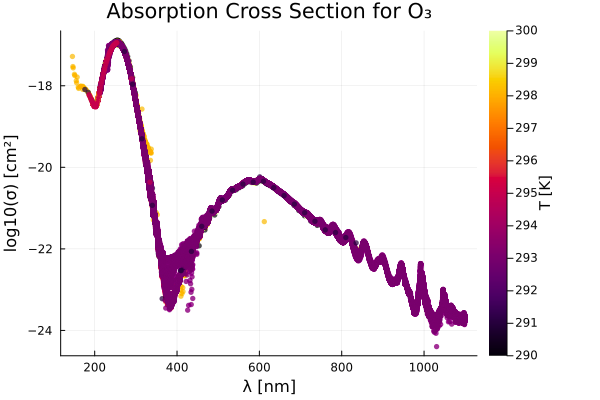
\includegraphics[width=0.85\columnwidth]{heart-chamber/photolysis/o3/cross-section/o3-data.png}
  \caption{The collected absorption cross section data for Ozone, $\mathrm{O_3}$, across a variety of temperatures.}
  \label{fig:cs-o3-data}
\end{figure}
As we can see, the bulk of the available data are for temperatures near the range $292-295$ Kelvin with a few sparse records at higher and lower temperatures. Because the Gaussian Process Regression model requires the Cholseky decomposition of a kernel matrix of size $N\times N$ ($N$ being the number of data records), we first perform a representative sub-sampling to generate a suitable train/test partition. The distribution of these records is illustrated in Figure \ref{fig:cs-o3-repr}.
\begin{figure}[!hbt]
  \centering
  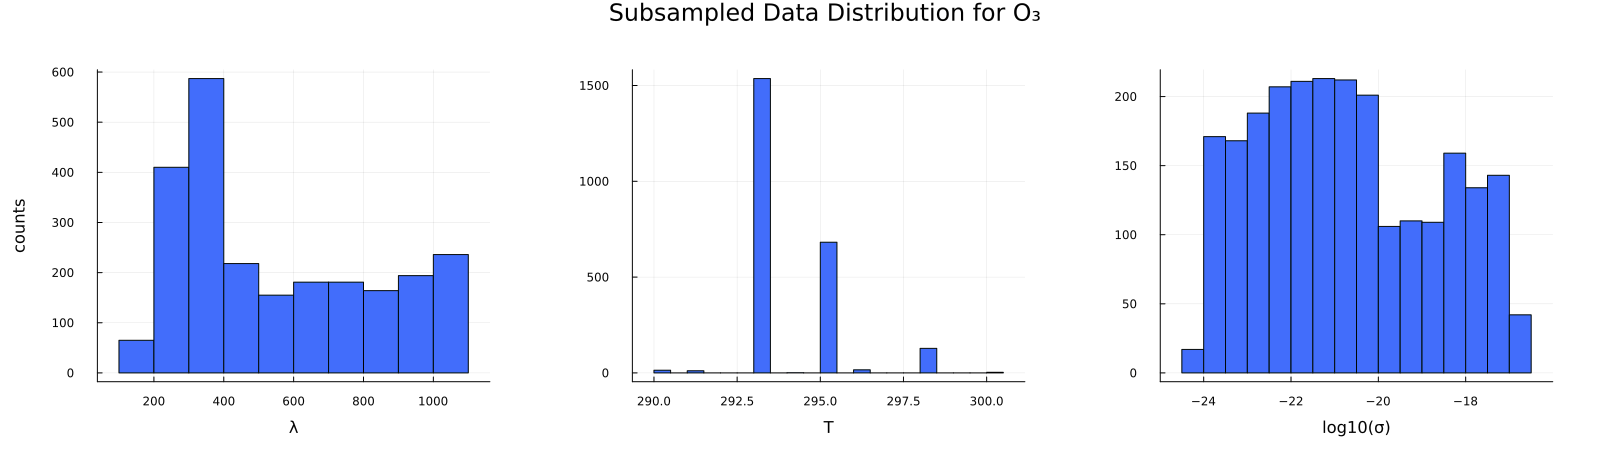
\includegraphics[width=0.9\columnwidth]{heart-chamber/photolysis/o3/cross-section/o3-representative-subsample.png}
  \caption{The distribution of subsampled $\mathrm{O}_3$ cross section data}
  \label{fig:cs-o3-repr}
\end{figure}

Using this dataset, we train a Gaussian Process Regression model to estimate $\log(\sigma)$. We fit the logarithm in order to make sure that the model learns the key absorption peaks since the values of $\sigma$ are observed to vary by multiple orders of magnitude. We chose to use a squared exponential kernel with hyperparameters for the variances as well as lengths scales for both $\lambda$ and $T$. Additionally, the mean value for the GPR is set to a default value of $-30$ to prevent spurious values from being estimated in wavelength regions of few records. A scatterplot evaluating the resulting fit is given in Figure \ref{fig:cs-o3-scatter}
\begin{figure}[!hbt]
  \centering
  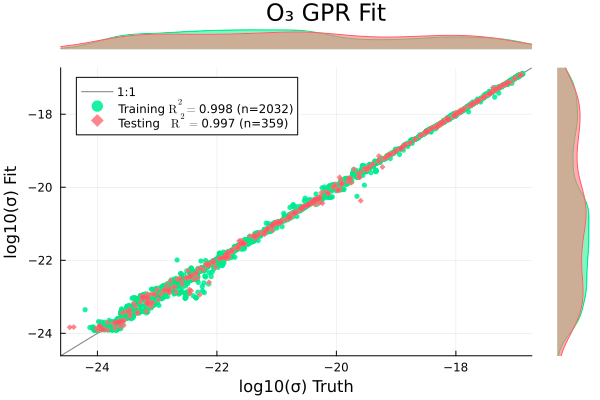
\includegraphics[width=0.85\columnwidth]{heart-chamber/photolysis/o3/cross-section/o3-gpr-scatter.png}
  \caption{A scatter plot of the resulting GPR fit evaluated on the training set (green) and a holdout testing dataset (red).}
  \label{fig:cs-o3-scatter}
\end{figure}
From this, we can clearly see that the model has done a good job fitting the collected data. Next, we use the model to predict $\sigma(T,\lambda)$ for a variety of temperatures as illustrated in Figure \ref{fig:cs-o3-pred}
\begin{figure}[h]
  \centering
  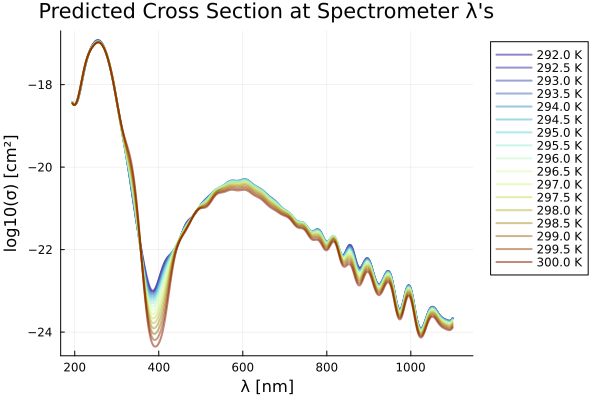
\includegraphics[width=0.85\columnwidth]{heart-chamber/photolysis/o3/cross-section/o3-prediction.png}
  \caption{Predicted $\mathrm{O_3}$ cross section as a function of temperature.}
  \label{fig:cs-o3-pred}
\end{figure}
These curves illustrate the temperature dependence of our GPR fit. For temperatures above $298$ K for which we had few records near $400$ nm, the model has biased towards the mean value of $-30$ (i.e. an effective cross section of $0$ cm\textsuperscript{2}. Because the data is sparse in this temperature range we should not implicitly trust the inferred values at high temperatures. To further illustrate this effect, we can plot the estimated cross section for two selected temperatures with uncertainty estimates obtained from the variance of the posterior distribution. An example of this is shown in Figure \ref{fig:cs-o3-fit-unc} below.
\begin{figure}[!hbt]
  \centering
  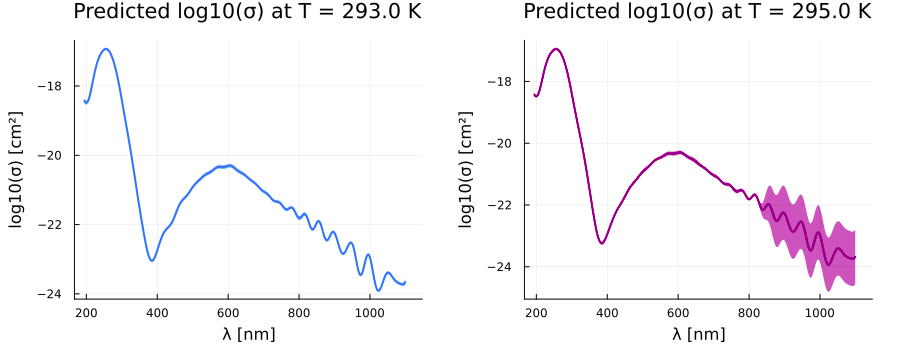
\includegraphics[width=0.85\columnwidth]{heart-chamber/photolysis/o3/cross-section/o3-prediction-uncertainty.png}
  \caption{Predicted $\mathrm{O_3}$ cross section for two temperatures with the associated uncertainty visualized. At $T=293$ K, we have many data points and therefore the associated fit uncertainty is small. For $T=295$ K, there are many fewer data points available above $800$ nm leading to a larger fit uncertainty.}
  \label{fig:cs-o3-fit-unc}
\end{figure}
The fit for $293$ Kelvin is well represented in the training data and therefore the associated uncertainty is low. For a temperature of $295$ K, there are few available measurements above $800$ nm, and consequently, the uncertainty estimated by our GPR is increased in this region (as we should hope).

\subsection{Quantum Yields}

To fit the quantum yield data, the procedure is nearly identical to that of the absorption cross section, however there is often far less data available for the quantum yield. As we shall demonstrate for the case of $\mathrm{O_3} + h\nu \longrightarrow \mathrm{O(1D)} + \mathrm{O_2}$, for regions where we do not have enough data to establish a suitable fit, we default to either a value of $1$ or $0$ depending on the region of wavelength space. Figure \ref{fig:qy-o3-data} illustrates the available quantum yield data for this reaction.
\begin{figure}[!hbt]
  \centering
  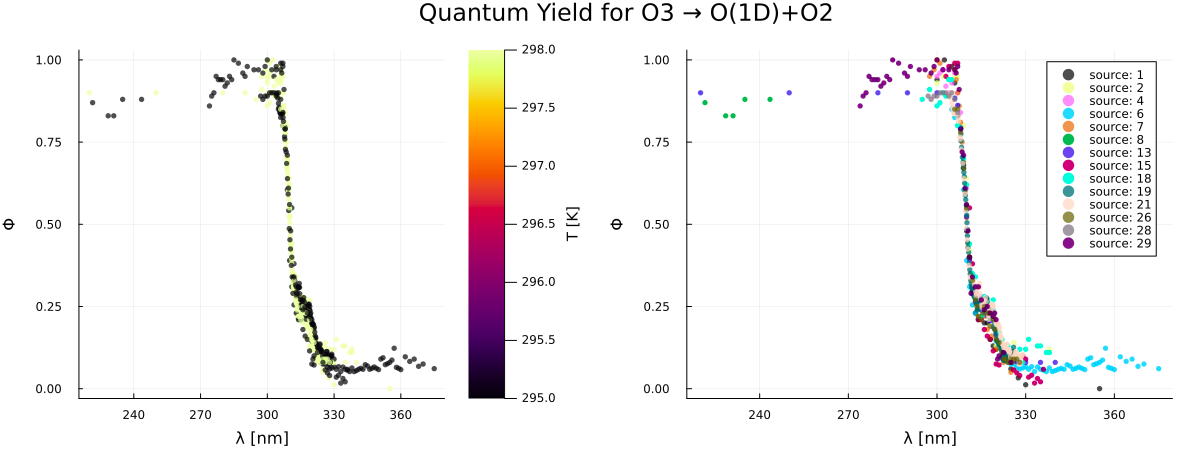
\includegraphics[width=0.95\columnwidth]{heart-chamber/photolysis/o3/quantum-yield/o3-qy-data.png}
  \caption{Data for the quantum yield of $\mathrm{O_3}$. Sources of data are far more sparse than for the absorption cross section.}
  \label{fig:qy-o3-data}
\end{figure}
In the panel on the left, we see that the quantum yield appears to have little temperature dependence. On the right we color the data points according to the reference they were scraped from. The distribution of the the data is illustrated in Figure \ref{fig:qy-o3-dist}.
\begin{figure}[!hbt]
  \centering
  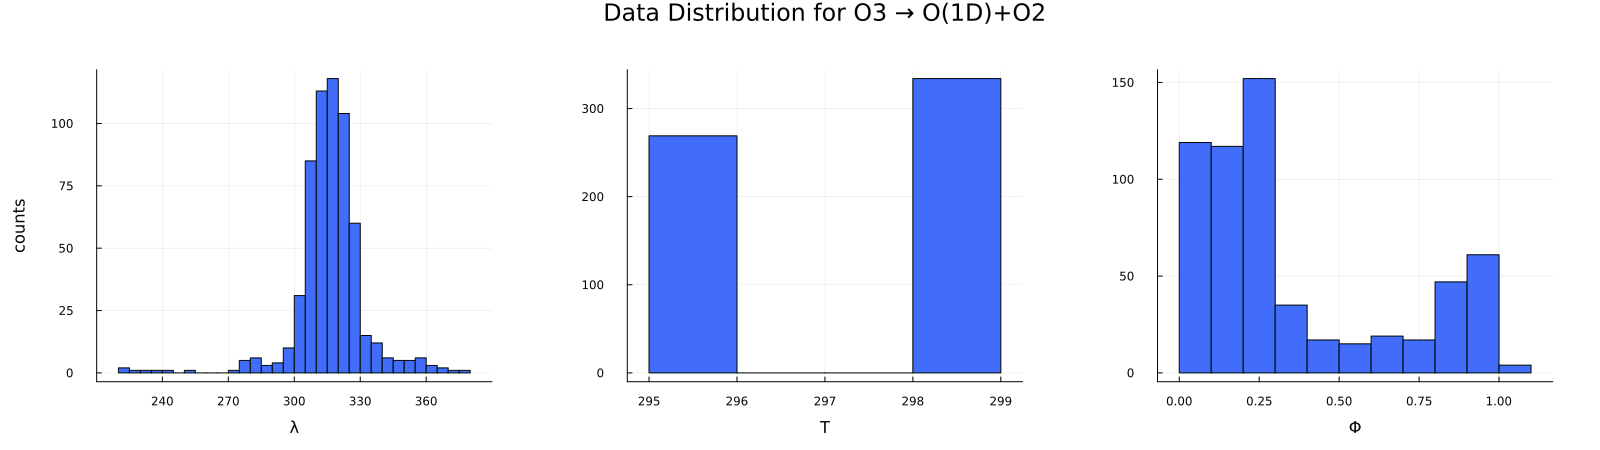
\includegraphics[width=0.95\columnwidth]{heart-chamber/photolysis/o3/quantum-yield/o3-qy-distribution.png}
  \caption{Distribution for the $\mathrm{O_3}$ quantum yield data.}
  \label{fig:qy-o3-dist}
\end{figure}
Here we see that the available data come from two temperatures and most of the wavelength dependence is estimated near steep drop in $\Phi$ between $300$ and $330$ nm.

The resulting GPR fit is evaluated in Figure \ref{fig:qy-o3-fit}.
\begin{figure}[!hbt]
  \centering
  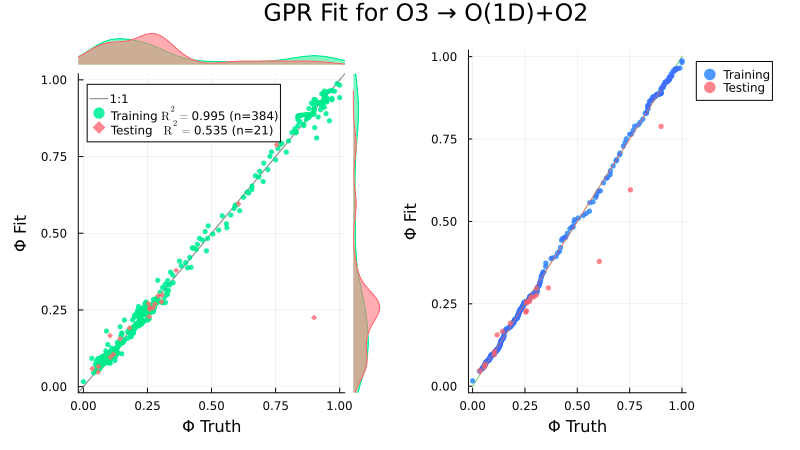
\includegraphics[width=0.95\columnwidth]{heart-chamber/photolysis/o3/quantum-yield/o3-qy-fit.png}
  \caption{Resulting GPR fit for $\mathrm{O_3}$ quantum yield data. Left: A scatter plot. Right: a quantile-quantile plot.}
  \label{fig:qy-o3-fit}
\end{figure}
It is obvious that we have far less data to fit, and as a consequence, we see in Figure \ref{fig:qy-o3-pred} that the model estimates a quantum yield of zero between $250$ and $270$ nanometers where there is a massive data gap. As we can not justify this drop on physical grounds, we construct a hybrid fit by interpolating between the estimates in these regions. For wavelengths below the first available datapoint, we default to a value of $1$. Similarly, for wavelengths beyond our last available record, we default to a value of $0$.
\begin{figure}[!hbt]
  \begin{subfigure}{.5\textwidth}
    \centering
    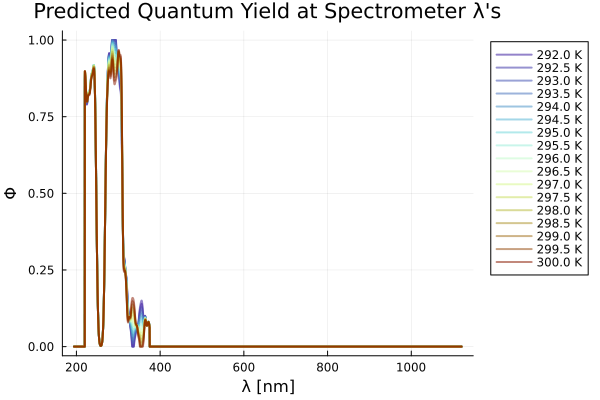
\includegraphics[width=0.85\columnwidth]{heart-chamber/photolysis/o3/quantum-yield/o3-qy-prediction.png}
    \caption{Predicted quantum yield for $\mathrm{O_3}$}
  \end{subfigure}
  \begin{subfigure}{.5\textwidth}
    \centering
    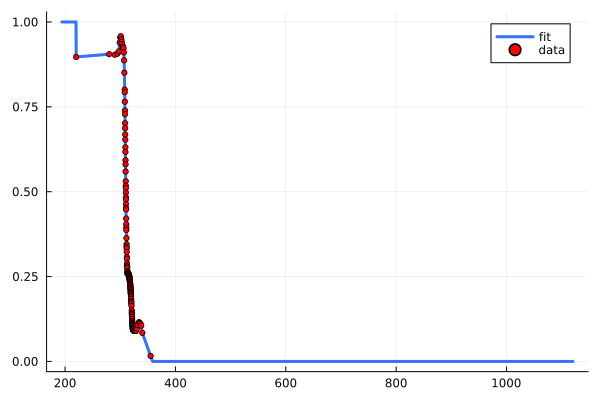
\includegraphics[width=0.85\columnwidth]{heart-chamber/photolysis/o3/quantum-yield/o3-qy-final.png}
    \caption{Final quantum yield estimates}
  \end{subfigure}
  \caption{Estimated quantum yields as a function of temperature and the resulting final fit.}
  \label{fig:qy-o3-pred}
\end{figure}


\subsection{Irradiance Spectra and Photolysis Rate Determination}

The last piece needed to estimate photolysis rates is the spectral irradiance. Using a calibrated Ocean Optics HR4000 UV-VIS spectrometer, we are able to measure the absolute irradiance spectrum every 15 seconds in units of $\mu\text{W}\cdot\text{cm}^{-2}\cdot\text{nm}^{-1}$. To obtain the desired units in terms of Photons, we utilize the plank relation $E(\lambda)=hc/\lambda$ to convert to $\text{Photons}\cdot{s}^{-1}\cdot\text{cm}^{-2}\cdot\text{nm}^{-1}$. A sample spectrum captured within an office building is shown in Figure \ref{fig:mean-irradiance}.
\begin{figure}[!hbt]
  \centering
  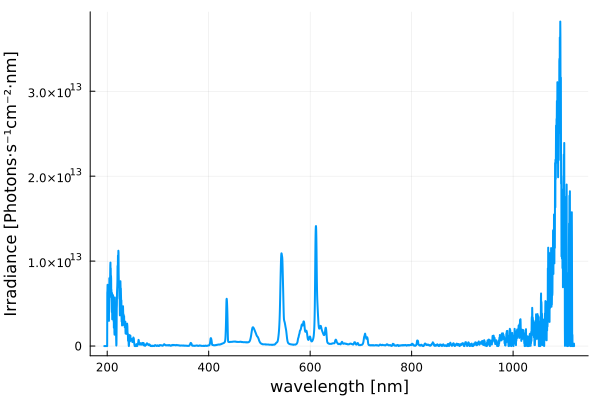
\includegraphics[width=0.7\columnwidth]{heart-chamber/photolysis/mean_irradiance.png}
  \caption{A plot of the spectral irradiance captured within a typical office building and averaged over 8 hours.}
  \label{fig:mean-irradiance}
\end{figure}

\subsection{Photolysis Rate Determination}

Finally, using numerical quadrature to integrate the measured irradiance spectrum together with the estimated absorption cross section and quantum yield, we are able to obtain the photolysis rate for each desired reaction. A comparison of all three quantities is provided in figure \ref{fig:photo-rate-example} from which we estimate a photolysis rate of ~$10^{-4}$ s.
\begin{figure}[!hbt]
  \centering
  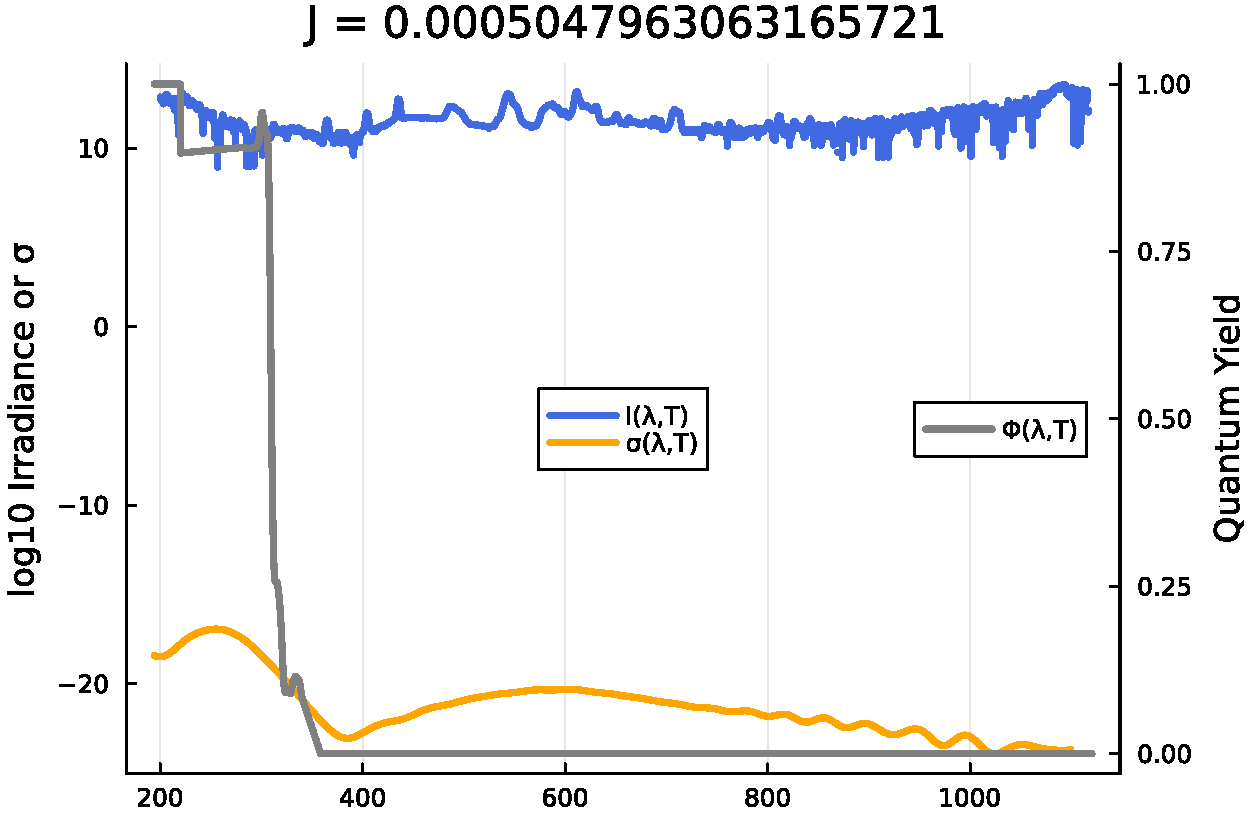
\includegraphics[width=0.7\columnwidth]{heart-chamber/photolysis/photolysis_plot.pdf}
  \caption{A comparison of the absorption cross section, quantum yield, and captured irradiance spectrum used to determine the photolysis rate for an $\mathrm{O_3}$ photolysis channel.}
  \label{fig:photo-rate-example}
\end{figure}



%% \section{HEART Chamber Data}

%% Initial data collected for evaluation of different PCO configurations.

%% \begin{figure}[h]
%%   \centering
%%   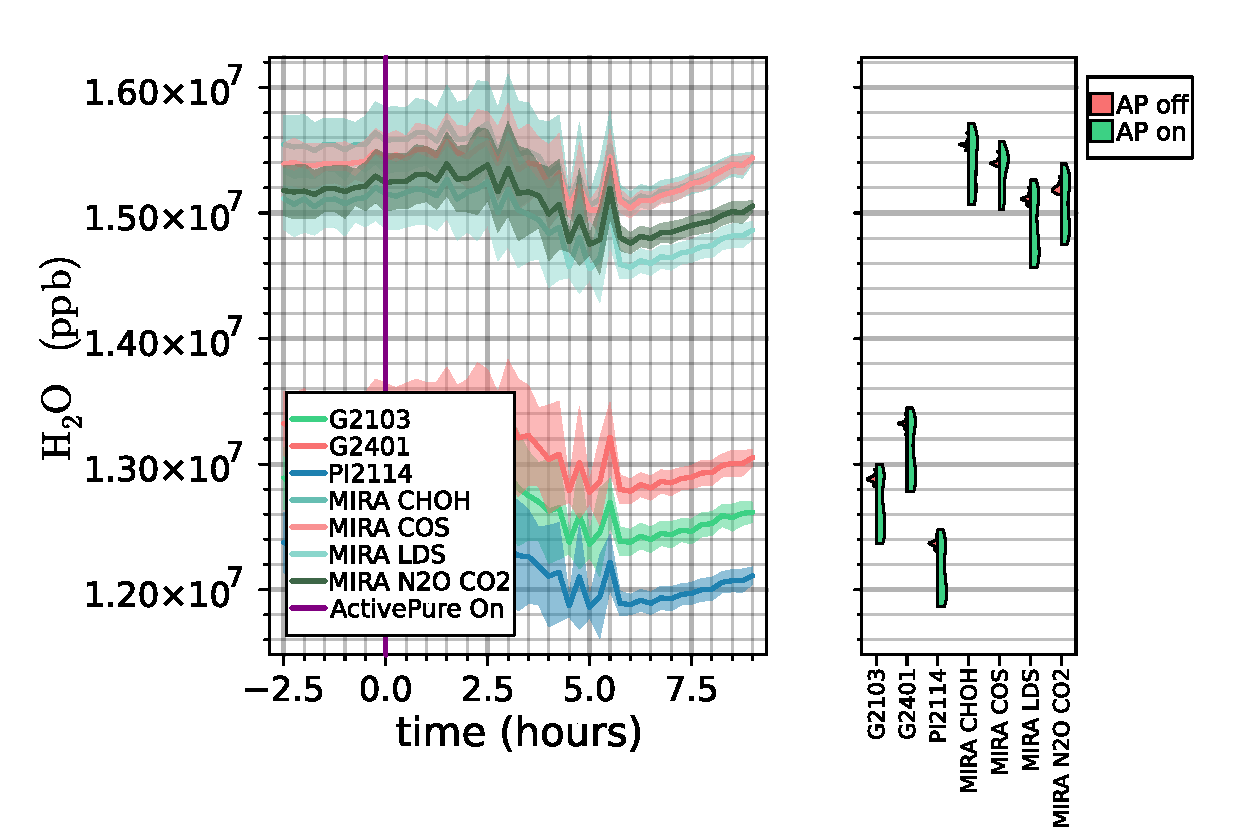
\includegraphics[width=0.85\columnwidth]{heart-chamber/instrument-measurements/H2O.pdf}
%% \end{figure}

%% \begin{figure}[h]
%%   \centering
%%   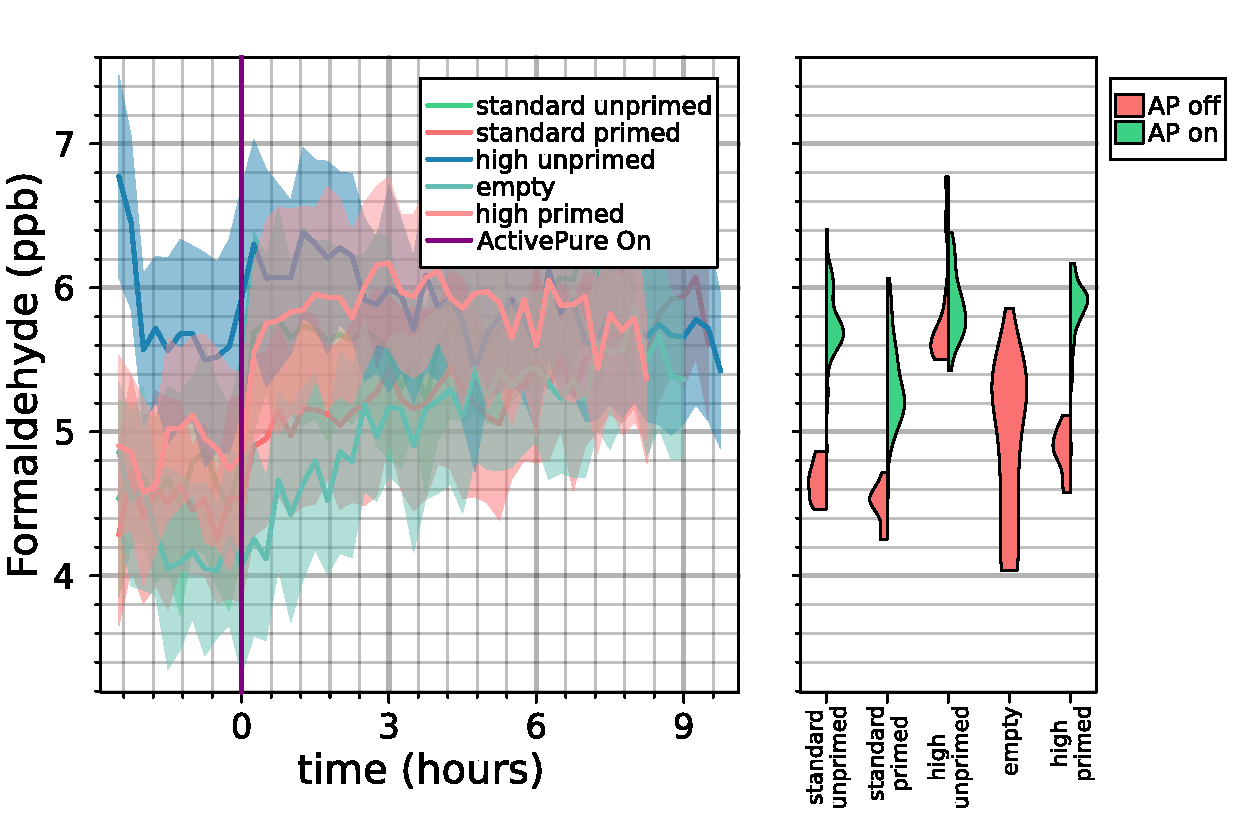
\includegraphics[width=0.85\columnwidth]{heart-chamber/instrument-measurements/formaldehyde.pdf}
%% \end{figure}


%% The $\mathrm{H_2O_2}$ is a good demonstrate of a high uncertainty instrument close to the detection limits.
%% \begin{figure}[h]
%%   \centering
%%   \includegraphics[width=0.85\columnwidth]{heart-chamber/instrument-measurements/H2O2.pdf}
%% \end{figure}

%% \begin{figure}[h]
%%   \centering
%%   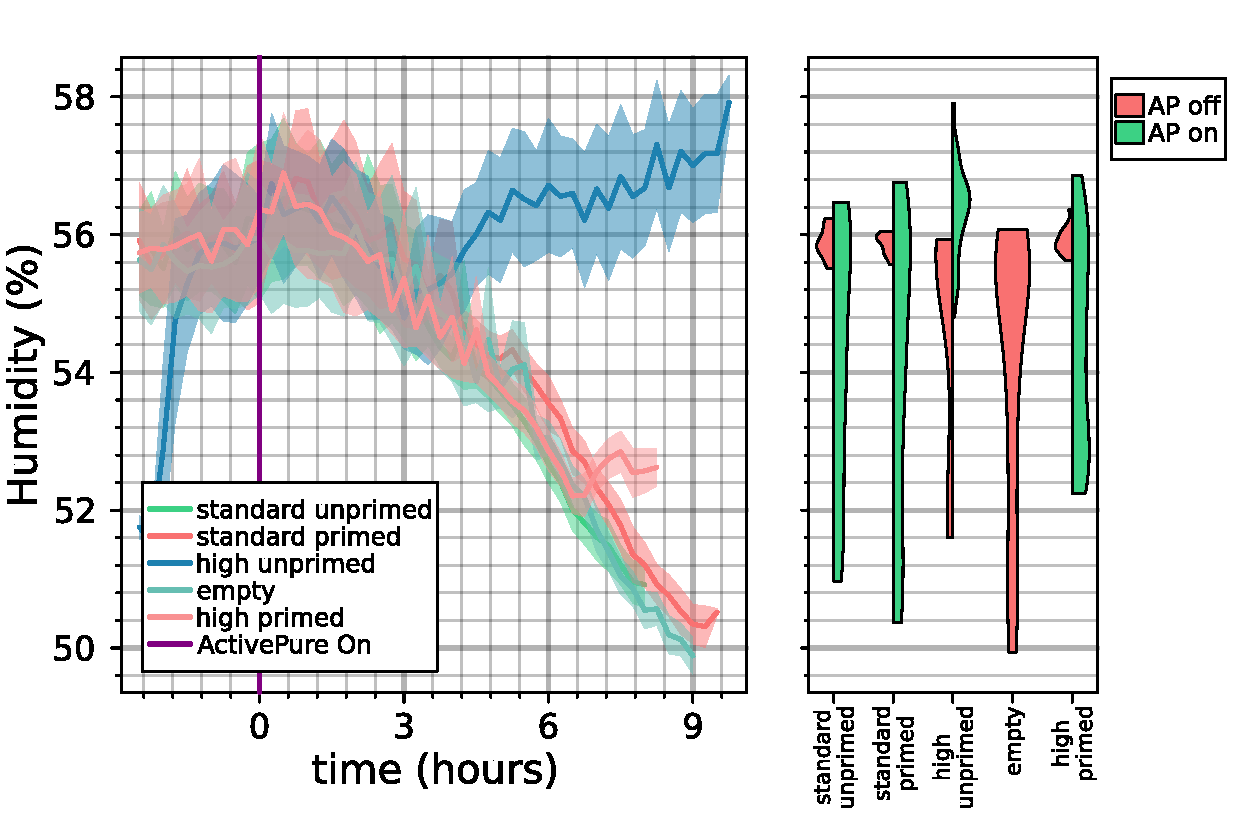
\includegraphics[width=0.85\columnwidth]{heart-chamber/instrument-measurements/humidity.pdf}
%% \end{figure}

%% \begin{figure}[h]
%%   \centering
%%   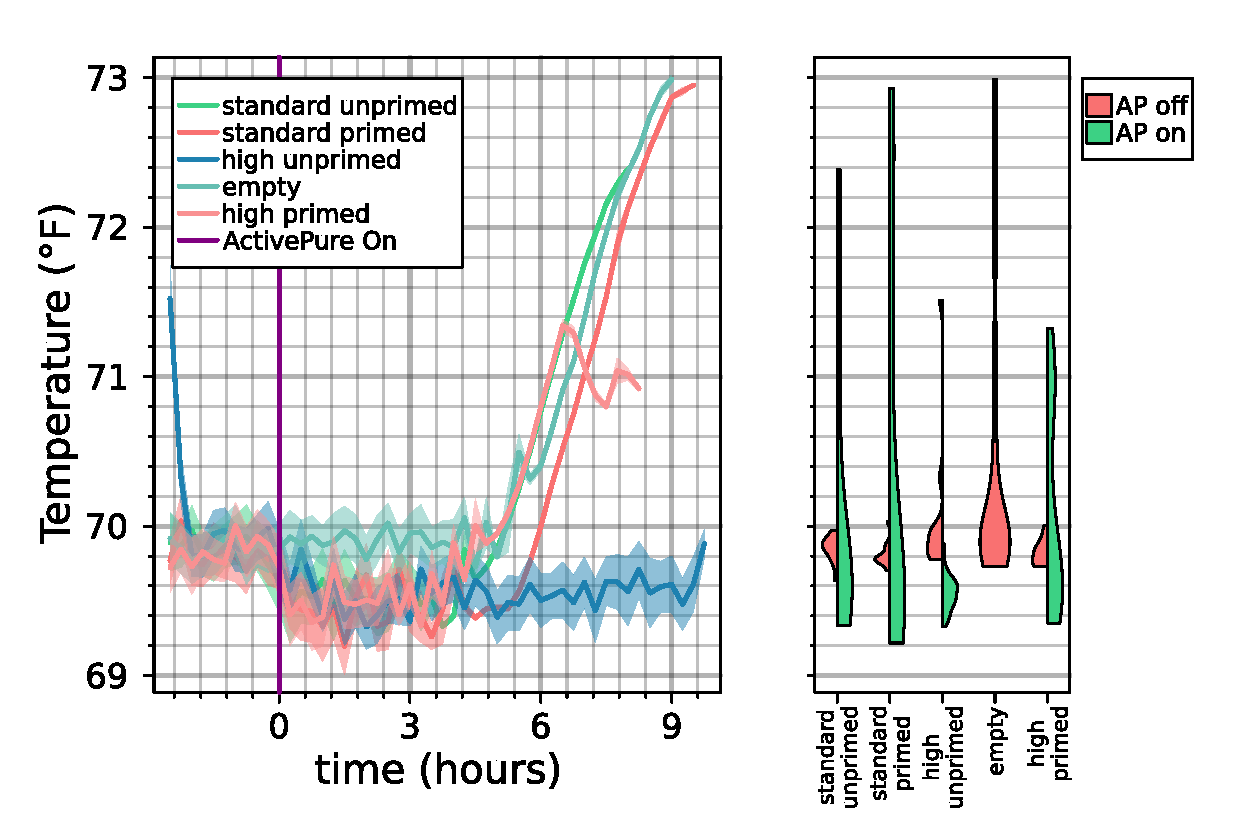
\includegraphics[width=0.85\columnwidth]{heart-chamber/instrument-measurements/temperature.pdf}
%% \end{figure}

%% \begin{figure}[h]
%%   \centering
%%   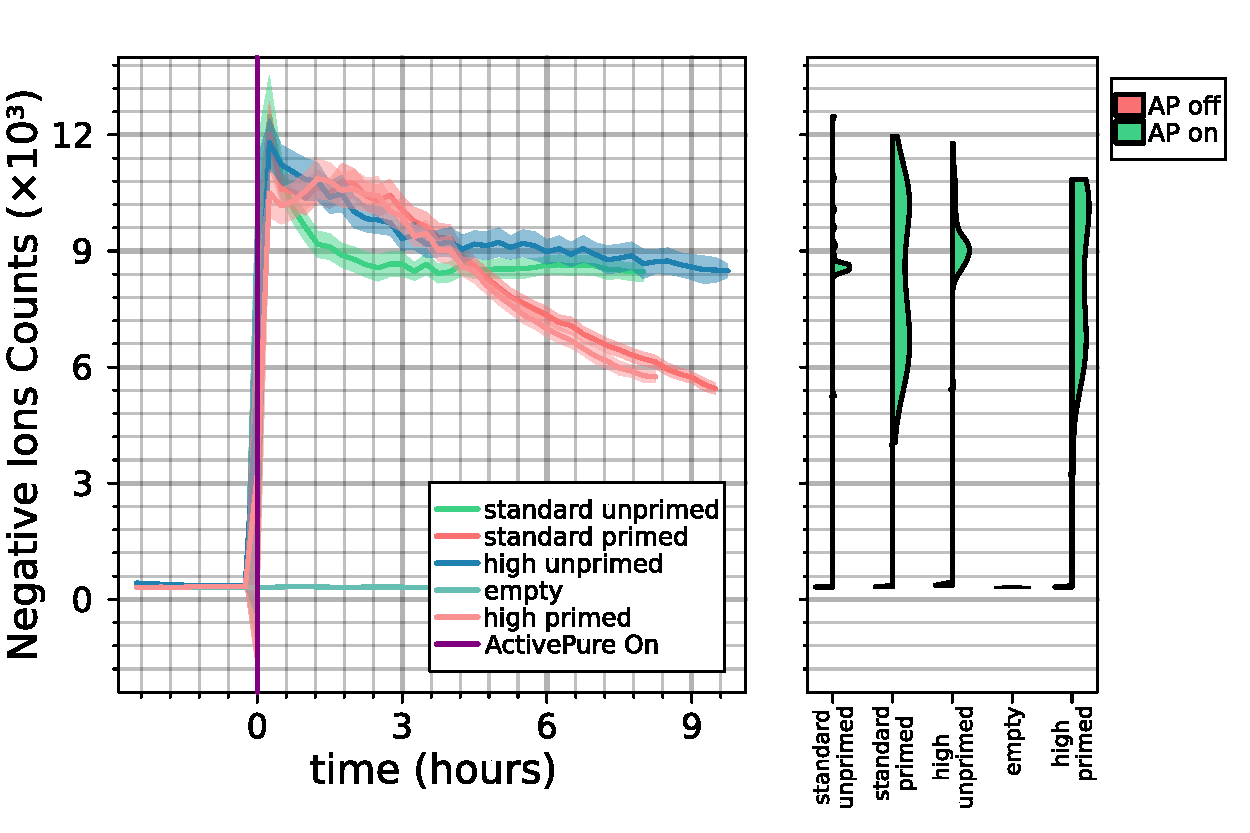
\includegraphics[width=0.85\columnwidth]{heart-chamber/instrument-measurements/negative_ions.pdf}
%% \end{figure}


\section{Chemical Data Assimilation}

In this section we present preliminary results from our chemical data assimilation model. The underlying chemical mechanism is an extension of \textit{AutoChem}, a NASA release software from David Lary \cite{Lary1999a, Lary2003a} augmented with reactions from the \textit{Master Chemical Mechanism} \cite{mcm-v3}. Together this yields a reactive system of over $5000$ chemical species and $16,000$ chemical reactions. The preliminary results discussed in this section have been carried out for a subset of the full mechanism consisting of ~1000 critical reactions including relevant ion chemistry. For computational efficiency, we have developed the code using the Julia programming language to take advantage of the cutting-edge differential equations suite, \texttt{DifferentialEquations.jl} which provides optimized solvers for the large, stiff systems encountered in our chemical mechanism \cite{differentialequations.jl}.

To develop our data processing pipeline and the associated assimilation code for use with the HEART chamber described in chapter 2, we have collected an initial data set using a subset of our sensors to sample the ambient air within the room. These include a variety of gas sensors for $\mathrm{CO_2}$, $\mathrm{NO_x}$, $\mathrm{O_3}$, $\mathrm{H_2O_2}$, $\mathrm{H_2O}$, and others in addition to ambient temperature and air pressure measurements. Data were collected over an ~8 hour period providing over 1 million individual records.

The first step of the assimilation pipeline is to apply the 4d-var algorithm outlined in chapter 3 in order to estimate reasonable initial conditions for all species integrated in the mechanism. These values are initialized using typical atmospheric values provided by the Master Chemical Mechanism together with the initial samples from our instruments. Figure \ref{fig:4d-var}
\begin{figure}[!hbt]
  \centering
  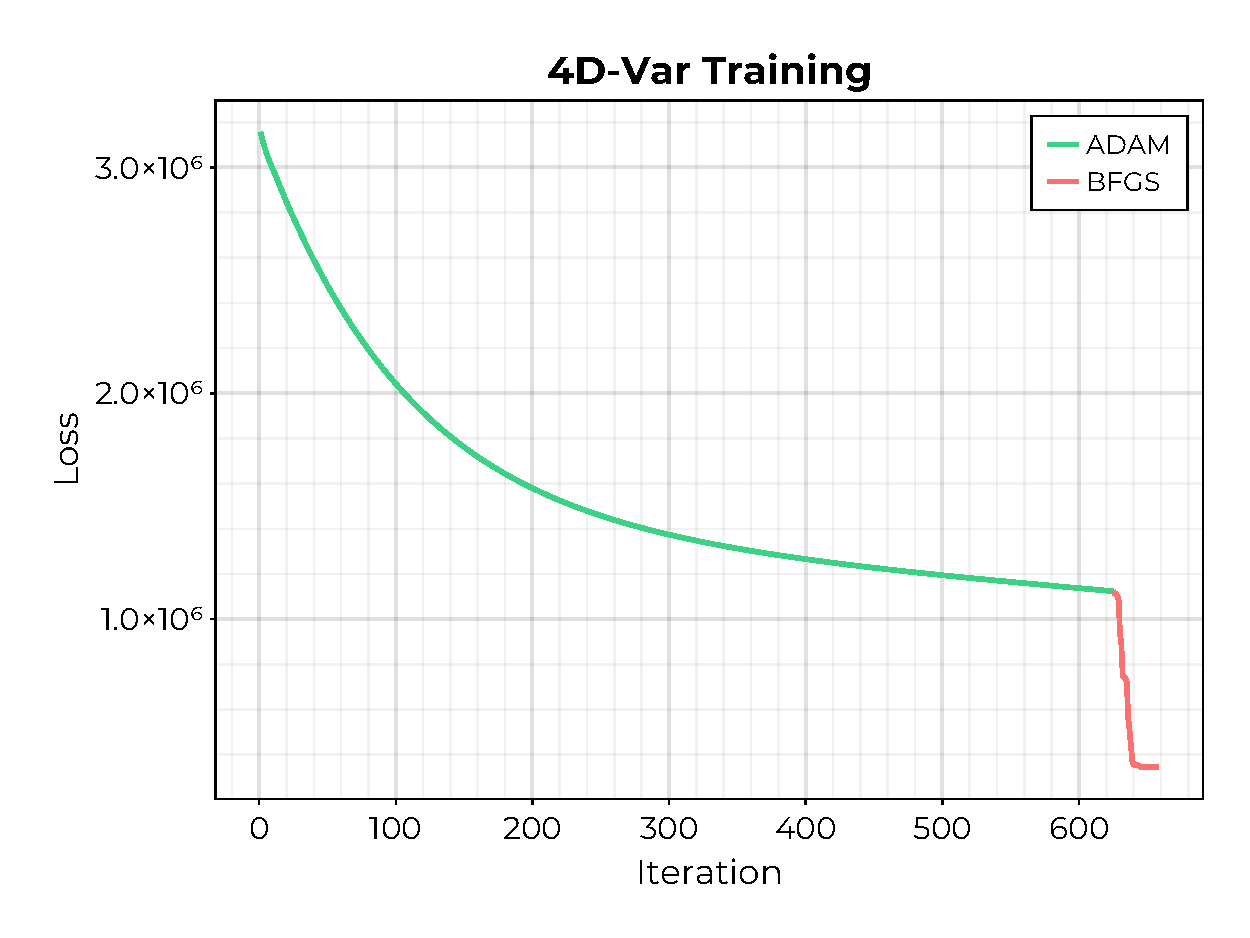
\includegraphics[width=0.85\columnwidth]{heart-chamber/assimilation/4dvar/losses.pdf}
  \caption{Training losses for 4d-var applied to our initial data collection.}
  \label{fig:4d-var}
\end{figure}
A two stage training procedure was utilized starting with the ADAM optimizer which is known to converge rapidly. A second, final round of optimization is then performed using the BFGS optimizer to make sure we are not stuck in a local minimum.

Next, the Ensemble Kalman Filter is used to integrate the starting concentrations estimated by the 4d-var step forward in time. At each instance where we have a measurement, the EKF algorithm adjusts the current concentrations to minimize the difference between simulation and data with consideration for the uncertainties of each. This allows for the simulation to remain valid over long integration periods \textit{and} makes it possible to infer the time-dependent concentrations of chemical species which we do not measure directly. Figure \ref{fig:h2o2} illustrates the time series of $\mathrm{H_2O2}$  as a volumetric mixing ratio in parts-per-trillion (ppt).
\begin{figure}[!hbt]
  \centering
  \includegraphics[width=0.85\columnwidth]{heart-chamber/assimilation/EKF/H2O2.pdf}
  \caption{Assimilation results for $\mathrm{H_2O_2}$.}
  \label{fig:h2o2}
\end{figure}
The gas analyzer producing the $\mathrm{H_2O_2}$ concentrations are close to the detection limits as evidenced by the large error bars. However, due to the propagation of information between chemical species by the EKF algorithm, the estimated analysis uncertainty is actually reduced as visualized by the colored ribbon around each estimate.

Figure \ref{fig:hcho} illustrates similar time series obtained for the concentration of formaldehyde ($\mathrm{HCHO}$).
\begin{figure}[!hbt]
  \centering
  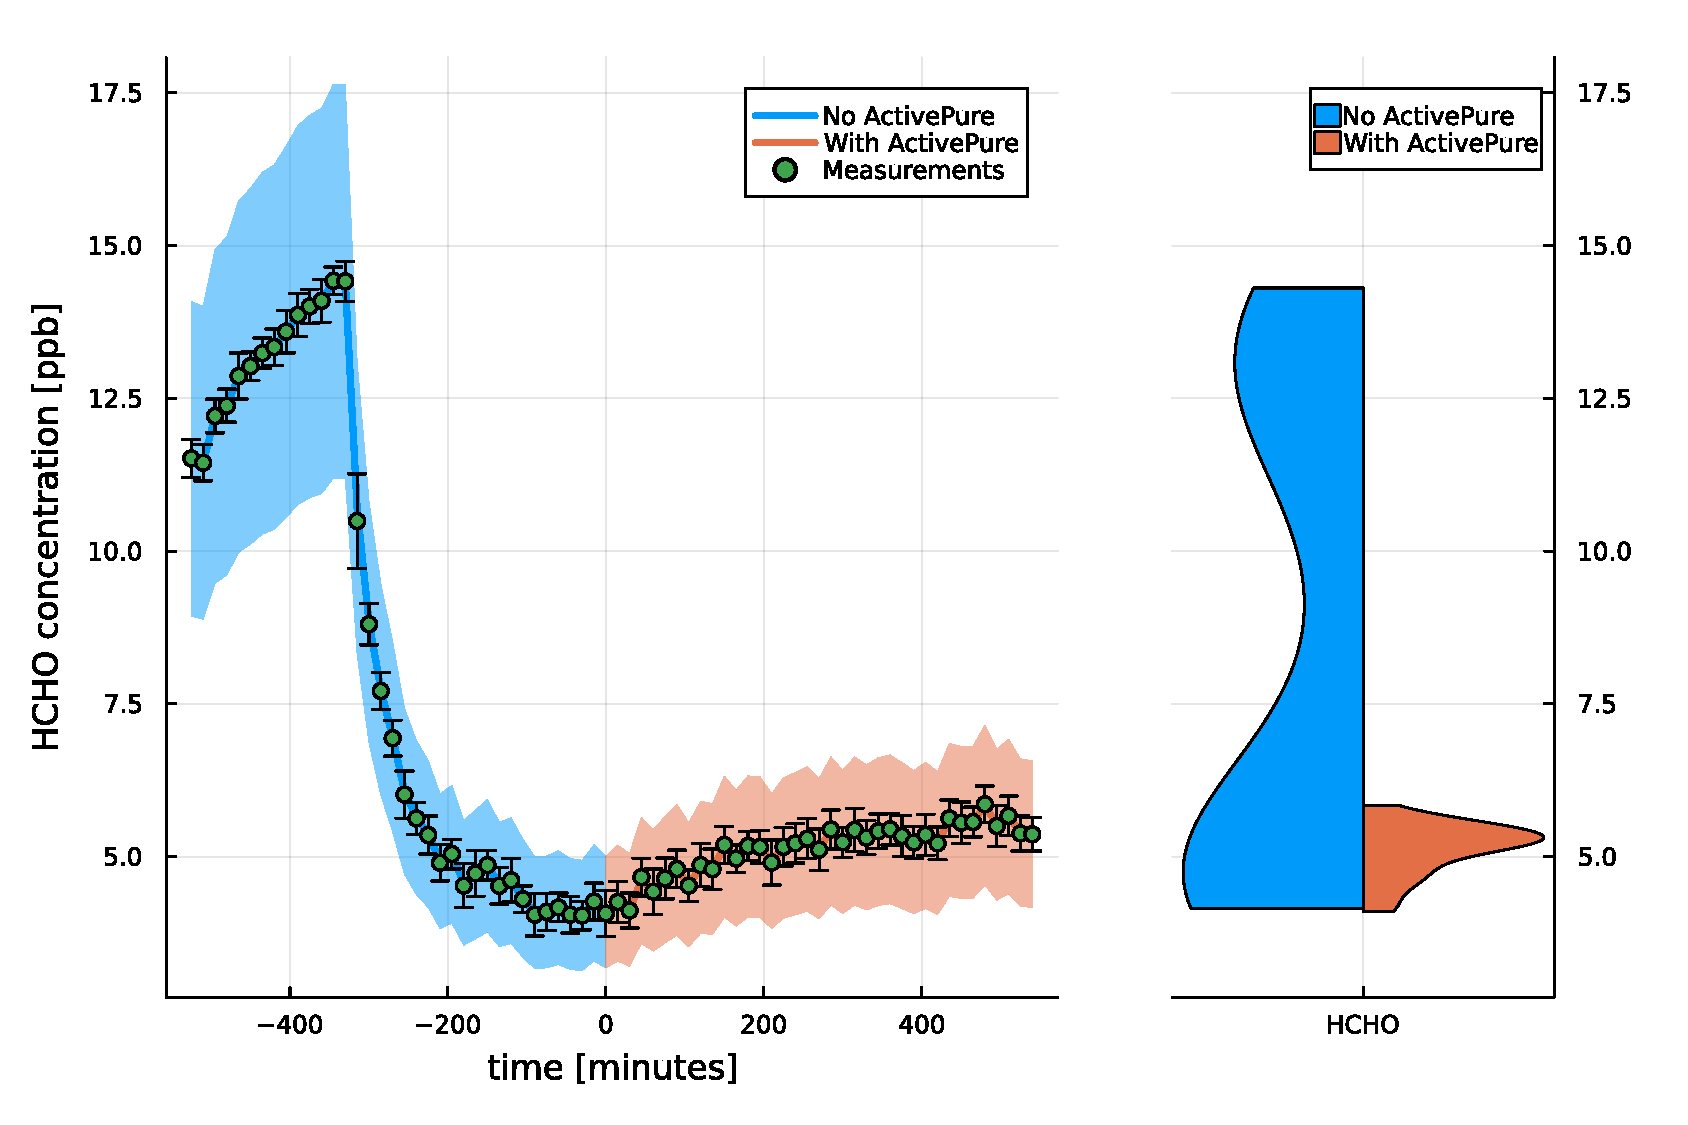
\includegraphics[width=0.85\columnwidth]{heart-chamber/assimilation/EKF/HCHO.pdf}
  \caption{Assimilation results for formaldehyde.}
  \label{fig:hcho}
\end{figure}
For this species, the analysis is able to follow the measurements however the assimilation has resulted in increased uncertainty estimates.


Finally, in Figure \ref{fig:oh} we show the time series of concentrations for the highly reactive hydroxyl radical, $\mathrm{OH}$.
\begin{figure}[!hbt]
  \centering
  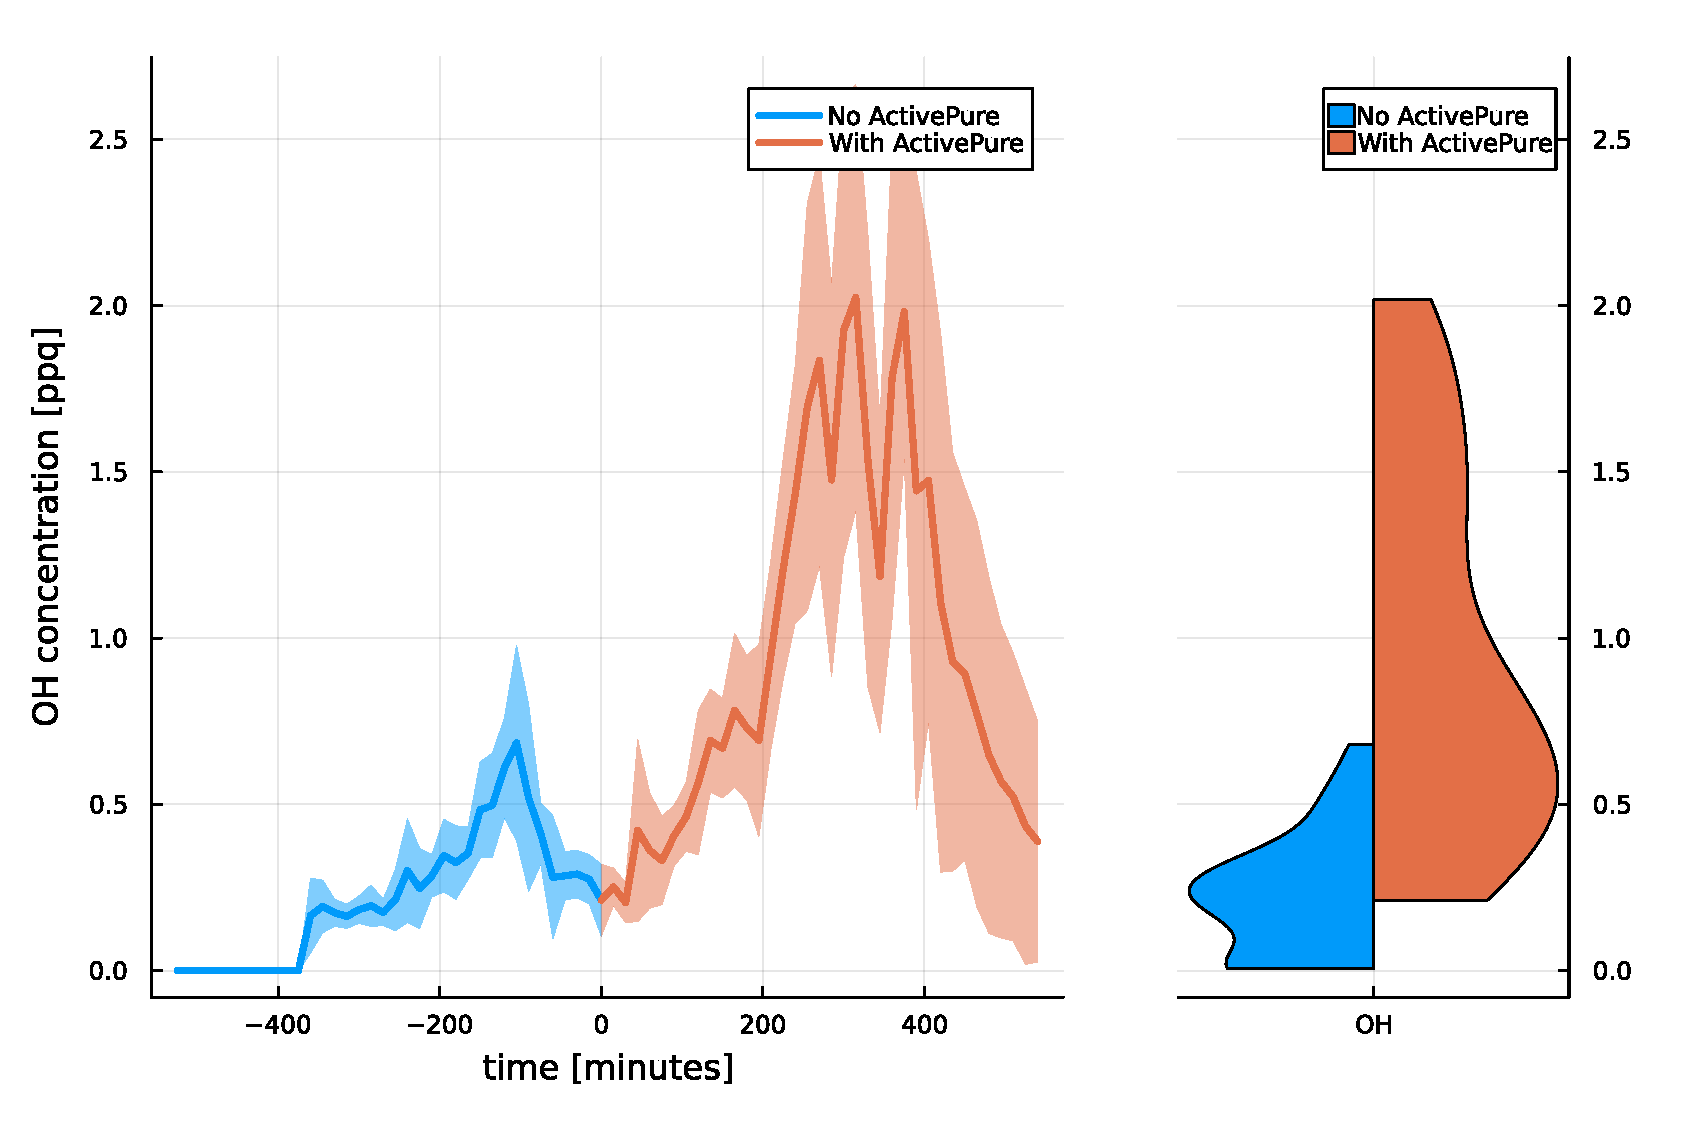
\includegraphics[width=0.85\columnwidth]{heart-chamber/assimilation/EKF/OH.pdf}
  \caption{Assimilation results for the hydroxyl radical $\mathrm{OH}$}
  \label{fig:oh}
\end{figure}
The hydroxyl radical is a highly reactive oxygen species which is difficult to measure directly due to its short lifetime (it tends to react with ~50 molecular diameters). Using this assimilation framework we are able to infer the abundance of $OH$ in the ambient room to be at the scale of a few parts-per-quadrillion.

The code for this project is made freely available at \url{https://github.com/john-waczak/AutoChem.jl}. A list of the reactions used in this preliminary investigation and their associated reaction rate coefficients are listed in Appendix A.

\section{Next Steps}

The next steps for this project include the following:
\begin{enumerate}
\item Extending the mechanism to include heterogeneous (mixed phase) reaction types.
\item Extending mechanism to include fixed rate surface deposition.
\item Development of a cd-EKF code for better uncertainty estimation.
\item Perform fixed temperature/pressure long time integration tests per the Boldi thesis to evaluate agreement with predictions from equilibrium thermodynamics.
\item Update reaction rates with recent JPL Kinetic evaluations.
\end{enumerate}

%% \section{An Evaluation of Photocatalytic Ionization}



%% \begin{itemize}
%% \item sensor fusion
%% \item photolysis
%% \item docker ingestion framework
%% \item Master Chemical Mechanism
%% \item CRI Mechanism
%% \item AutoChem
%% \item data assimilation
%% \item Overview of all sensor in sensor matrix
%% \item Overview of measurement capabilities (list of species, uncertainty levels, etc...)
%% \item Overview of containerized data acquisition pipeline
%% \item NodeRed
%% \item InfluxDB
%% \item Grafana
%% \item Quarto
%% \item Automatic Alerts
%% \item Automatic Reports
%% \item MCM Implementation in Julia
%% \item Direct computation of Photolysis rates
%% \item Combination with Dr. Lary's AutoChem
%% \item Addition of Ion Chemistry from MIT Lightning disseration
%% \item Visualization of chemical cycles
%% \item SciML methods to infer below detection limits
%% \item Ion Chemistry
%% \item Indoor Air Quality
%% \item Photocatalytic Ionization
%% \end{itemize}


